\documentclass[11pt,a4paper]{article}
\usepackage[margin=2.5cm]{geometry}
\usepackage[utf8]{inputenc}
\usepackage[T1]{fontenc}
\usepackage{hyperref}
\renewcommand{\familydefault}{\sfdefault}
\usepackage{helvet}
\pagestyle{empty}
\usepackage[kerning=true]{microtype}
\usepackage{parskip}
\usepackage{sansmath}
\usepackage[font={small, bf}]{caption}
\usepackage[font={small}]{subcaption}
\usepackage{graphicx}
\usepackage{multicol}
\setlength{\abovecaptionskip}{0pt}
\setlength{\floatsep}{10pt}
\setlength{\textfloatsep}{0pt}
\setlength{\intextsep}{0pt}
\setlength{\belowcaptionskip}{0pt}
\setlength{\parindent}{5ex}
\setlength{\parskip}{0pt}
% Feel free to use additional packages for glosses, figures, whatnot.

% The next bit is for reserving sufficient space for authors,
% affiliations, and e-mail address.  No need to change for initial
% anonymous version.  For the final version, replace the
% \toggletrue{anonymous} with \togglefalse{anonymous} to de-anonymize.
\usepackage{etoolbox}
\newtoggle{anonymous}
\toggletrue{anonymous}

\renewcommand{\title}[1]{\textbf{#1}\\}
\newcommand{\authors}[1]{\iftoggle{anonymous}{\phantom{#1}}{#1}\\}
\newcommand{\email}[1]{\iftoggle{anonymous}{\phantom{#1}}{#1}}

\begin{document}

% First page:

% Insert title, authors, affiliations, and e-mail address in the next three lines:

\title{TODO}
\authors{Veronica Boyce (Stanford), Roger Hawkins (Princeton), Noah Goodman (Stanford), Michael C. Frank (Stanford)} 
\email{vboyce@stanford.edu}
\newline
%

% Intro
%TODO citations
Shared referring expressions are a necessity for efficient communication; when there are not widely shared conventional names for objects, people must create spontaneous ad-hoc expressions. The formation and adoption of these new reference expressions is well-studied in dyadic contexts where one speaker refers to a set of images repeatedly to one listener. Over repetition, a few key phenomena emerge: listener's have high and increasing target accuracy while speaker's descriptions shorten as nicknames develop; crucially, these reduced referring expressions are partner-specific; dyads converge to nicknames, but dyads diverge from other dyads. 

% The hole

This leaves a question of how well it generalizes to larger groups and what properties of the communication channel are necessary for the pattern to emerge. We explore this with a 2x2 experiment: with 2-person groups and 6-person groups and either thick or thin communication channels. In the *thick* channel, the same person is the speaker throughout, speakers and listeners all use a shared chat to communicate, and TODO feedback. In contrast, in the *thin* condition, the speaker role rotates, only the speaker can write chat messages, the listener backchannel is limited to sending 4 emojis to indicate their confusion or comprehension, and TODO feedback. 
%TODO crib from pre-reg 

We recruit participants from Prolific to do this experiment as a real-time interactive game written in Empirica CITE. Participants see 12 tangram figures, one of which is indicated to the speaker, who describes the target to the listeners, who click on their selection. At the end of the trial feedback is given.  After all 12 tangrams have been described, the process repeats, for a total of 6 blocks (72 referential trials). We had rouglhy 40 games in each of the 4 conditions, for a total of ZZZ participants. 

% Results
%TODO we have ZZ words
This study generates rich linguistic dialogues. Here we report 4 key results. 

1) Accuracy: (see Fig) Consistent with prior work, listeners are overall relatively accurate to begin with and their accuracy increases over time. There are condition differences; listeners in the 2-person group are more accurate as are listeners in the thick channel condition. 

2) Reduction: We look at the amount of language the speaker produced for each tangram image. Over the course of blocks, the number of words produced decrease. Small games start out more efficient with language than larger groups, but they.

To analyze the content of the language, we embed the utterances with SBERT CITEME and then take the cosine similarties between embeddings as a measure for similarity between the references. 

3) We take cosine similarities between descriptions of the same tangram in the same block in different games. This is a measure of divergence between games. We find ...

4) TO measure convergence within games, we treat final round utterances as the "convention" and compare them to earlier references in the same game to the same tangram. We find ...

%TODO conclusion 

\newpage

\begin{figure}
	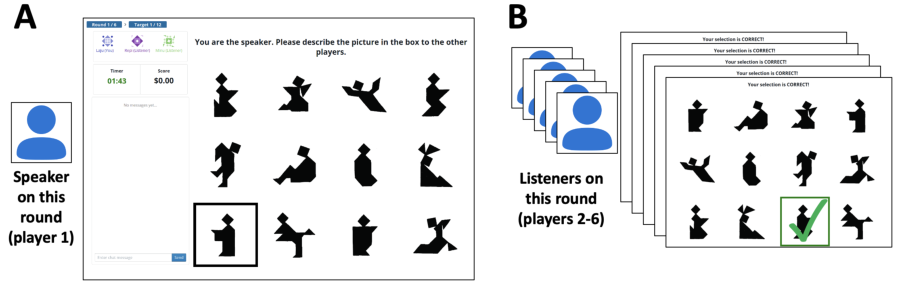
\includegraphics[width=\textwidth]{../images/interface-1.pdf}
	\caption{Schematic of player interface}{TODO! A. Speaker view B. Listener view}
\end{figure}

\begin{figure}
	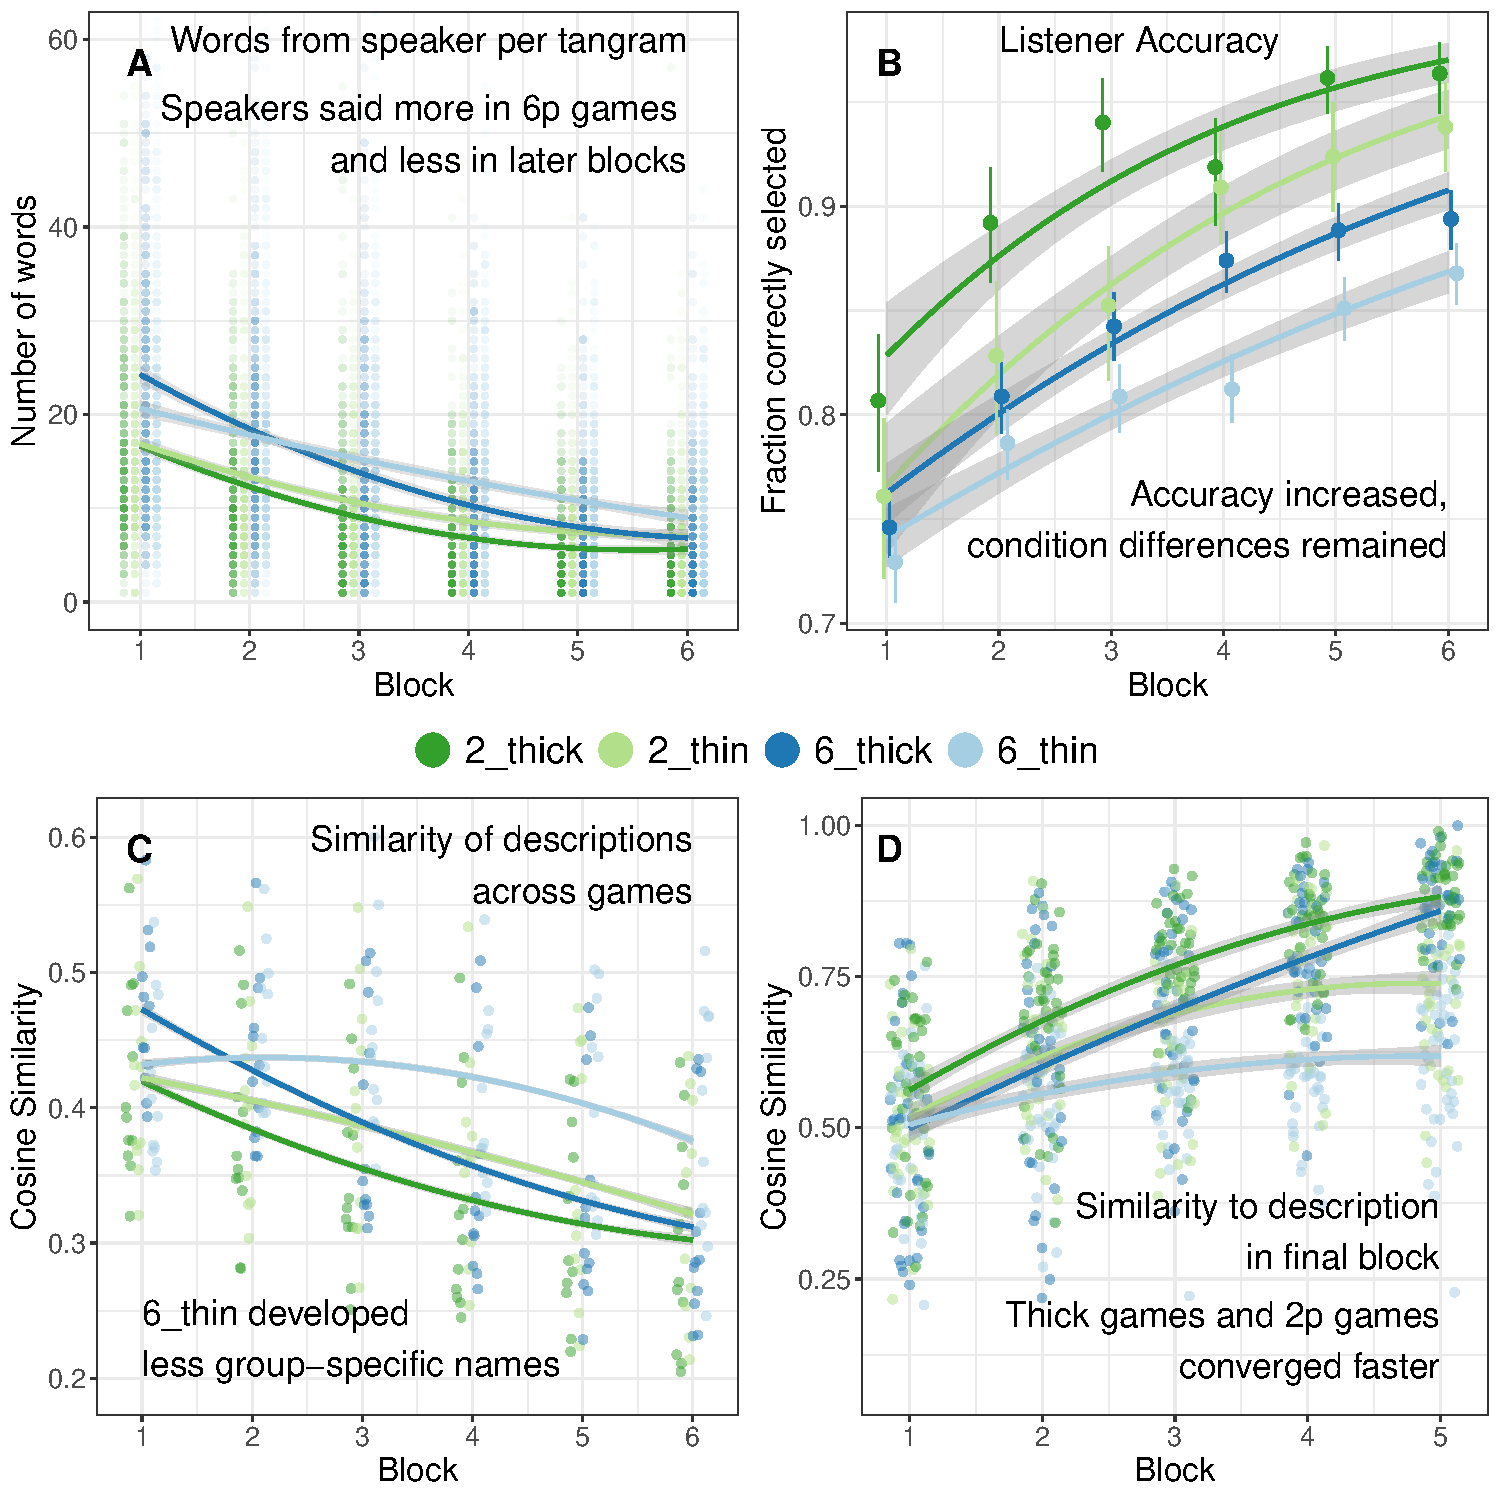
\includegraphics[width=\textwidth]{../images/CAMP1.pdf}
	\caption{Results by condition}{TODO}
\end{figure}

\begin{figure} Bibliography goes here \end{figure}

\end{document}